\documentclass[tikz,border=8mm]{standalone}
\usepackage[american]{circuitikz}
\begin{document}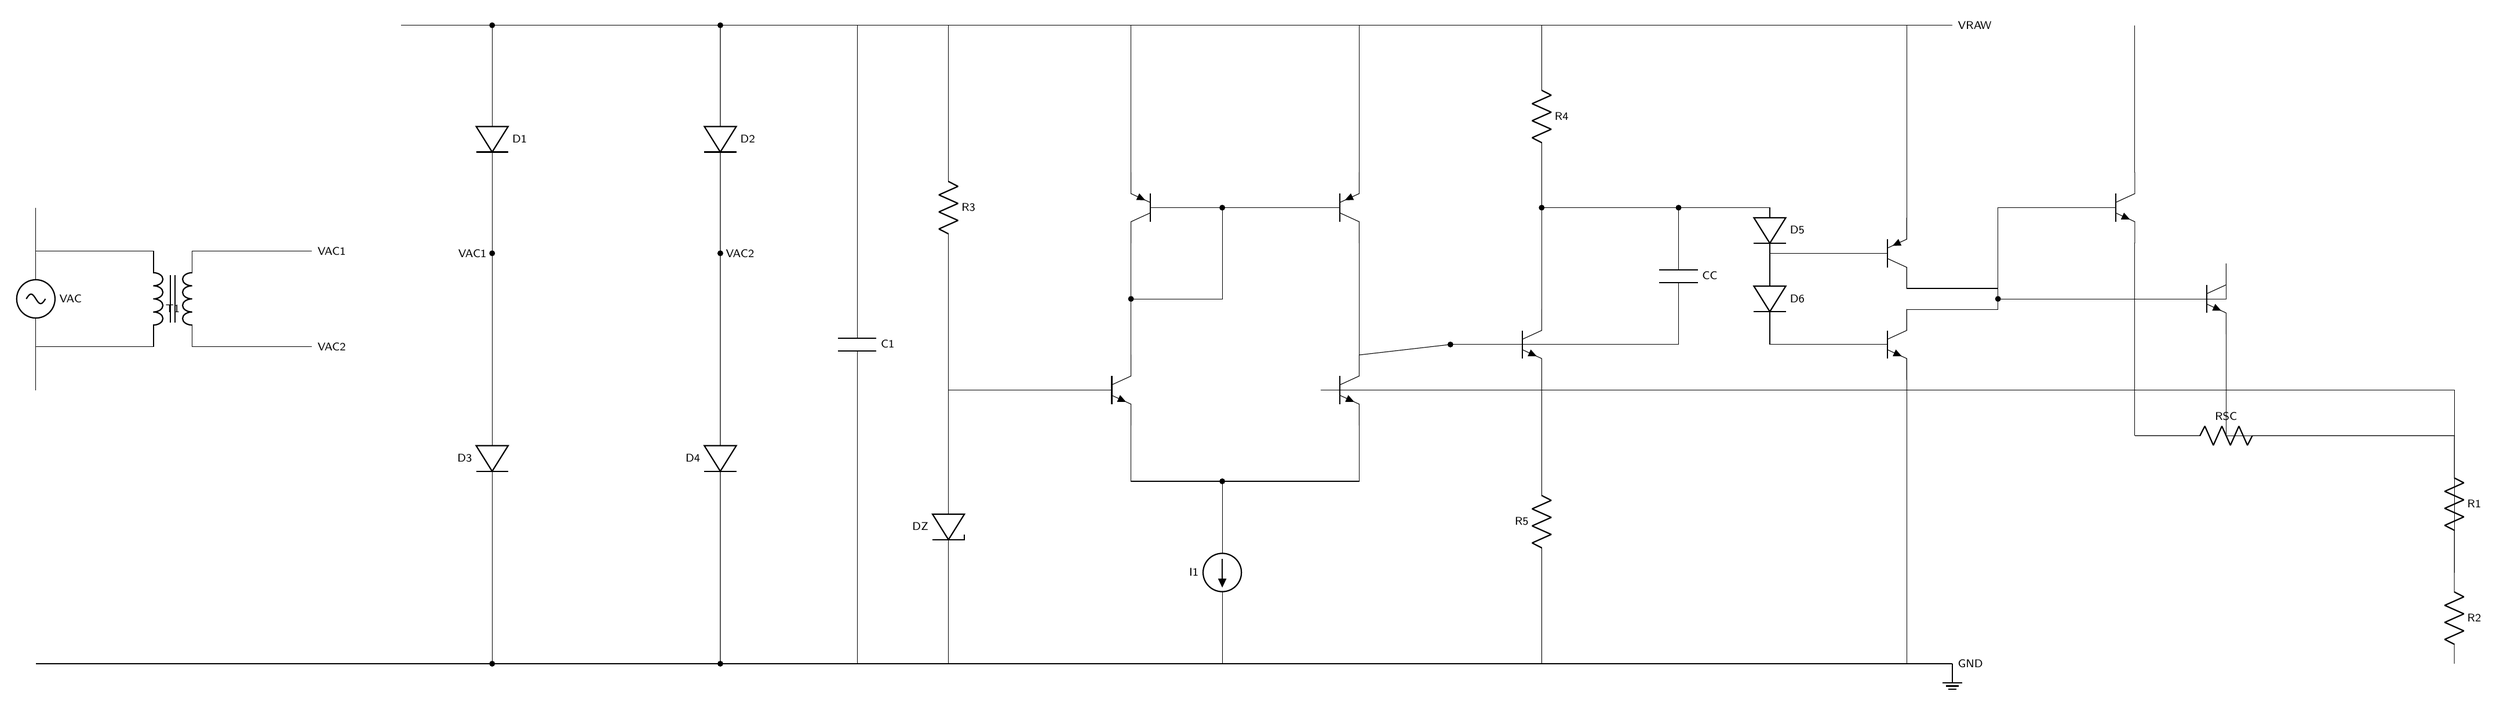
\begin{tikzpicture}[every node/.style={font=\sffamily\scriptsize}]
\draw(8,14)--(42,14)node[right]{VRAW};\draw(0,0)--(42,0)node[right]{GND};\draw(42,0)node[ground]{};
\node[transformer core](T1)at(3,8){};\node[below]at(T1){T1};\draw(0,10)to[sV,l=VAC](0,6);\draw(0,10)|-(T1.A1);\draw(0,6)|-(T1.A2);\draw(T1.B1)--++(2,0)node[right]{VAC1};\draw(T1.B2)--++(2,0)node[right]{VAC2};
\coordinate(A1)at(10,9);\coordinate(A2)at(15,9);\node[left]at(A1){VAC1};\node[right]at(A2){VAC2};\draw(10,14)to[D,l=D1](A1)to[D,l_=D3](10,0);\draw(15,14)to[D,l=D2](A2)to[D,l_=D4](15,0);\foreach\p in{(10,14),(10,9),(10,0),(15,14),(15,9),(15,0)}\draw\p node[circ,fill,inner sep=1pt]{};\draw(18,14)to[C,l=C1](18,0);
\coordinate(REF)at(20,6);\draw(20,14)to[R,l=R3](REF)to[zD,l_=DZ](20,0);\node[npn](Q1)at(24,6){};\node[npn](Q2)at(29,6){};\draw(REF)--(Q1.B);\draw(Q1.E)|-(24,4)--(29,4)-|(Q2.E);\draw(26,4)to[isource,l_=I1](26,0);\draw(26,4)node[circ,fill,inner sep=1pt]{};
\node[pnp,xscale=-1](Q3)at(24,10){};\node[pnp](Q4)at(29,10){};\draw(Q3.E)|-(24,14);\draw(Q4.E)|-(29,14);\draw(Q1.C)--(Q3.C);\draw(Q2.C)--(Q4.C);\draw(Q3.B)--(26,10)--(Q4.B);\draw(24,8)-|(26,10);\draw(24,8)node[circ,fill,inner sep=1pt]{};\draw(26,10)node[circ,fill,inner sep=1pt]{};
\coordinate(N2)at(31,7);\draw(Q2.C)--(N2);\draw(N2)node[circ,fill,inner sep=1pt]{};\node[npn](Q5)at(33,7){};\draw(N2)--(Q5.B);\coordinate(VAS)at(33,10);\draw(Q5.C)--(VAS);\draw(33,14)to[R,l=R4](VAS);\draw(Q5.E)to[R,l_=R5](33,0);\draw(VAS)--(36,10)to[C,l=CC](36,7)|-(N2);\draw(VAS)node[circ,fill,inner sep=1pt]{};\draw(36,10)node[circ,fill,inner sep=1pt]{};
\draw(VAS)--(38,10)to[D,l=D5](38,9)to[D,l=D6](38,7);\node[pnp](Q6)at(41,9){};\node[npn](Q7)at(41,7){};\draw(38,9)--(Q6.B);\draw(38,7)--(Q7.B);\draw(Q6.E)|-(41,14);\draw(Q7.E)|-(41,0);\coordinate(DRV)at(43,8);\draw(Q6.C)-|(DRV);\draw(Q7.C)-|(DRV);\draw(DRV)node[circ,fill,inner sep=1pt]{};\node[npn](Q8)at(46,10){};\draw(Q8.C)|-(46,14);\draw(DRV)|-(Q8.B);\coordinate(SENSE)at(46,5);\draw(Q8.E)|-(SENSE);\draw(SENSE)to[R,l=RSC](50,5);\coordinate(VOUT)at(50,5);\node[npn](Q9)at(48,8){};\draw(SENSE)|-(Q9.B);\draw(Q9.E)|-(VOUT);\draw(Q9.C)|-(DRV);\coordinate(FB)at(53,2);\draw(VOUT)--(53,5)to[R,l=R1](FB)to[R,l=R2](53,0);\draw(FB)|-(Q2.B);\end{tikzpicture}\end{document}
